\documentclass[8pt,aspectratio=169]{beamer}
\usetheme{Madrid}
\usepackage{graphicx,booktabs,adjustbox,multicol,amsmath,amssymb,listings,xcolor}
\definecolor{mlblue}{RGB}{0,102,204}
\definecolor{mlpurple}{RGB}{51,51,178}
\definecolor{mllavender}{RGB}{173,173,224}
\definecolor{mllavender2}{RGB}{193,193,232}
\definecolor{mllavender3}{RGB}{204,204,235}
\definecolor{mllavender4}{RGB}{214,214,239}
\definecolor{mlorange}{RGB}{255,127,14}
\definecolor{mlgreen}{RGB}{44,160,44}
\definecolor{mlred}{RGB}{214,39,40}
\definecolor{mlgray}{RGB}{127,127,127}
\definecolor{solkeyword}{RGB}{0,102,153}
\setbeamercolor{palette primary}{bg=mllavender3,fg=mlpurple}
\setbeamercolor{palette secondary}{bg=mllavender2,fg=mlpurple}
\setbeamercolor{palette tertiary}{bg=mllavender,fg=white}
\setbeamercolor{palette quaternary}{bg=mlpurple,fg=white}
\setbeamercolor{structure}{fg=mlpurple}
\setbeamercolor{title}{fg=mlpurple}
\setbeamercolor{frametitle}{fg=mlpurple,bg=mllavender3}
\setbeamercolor{block title}{bg=mllavender2,fg=mlpurple}
\setbeamercolor{block body}{bg=mllavender4,fg=black}
\setbeamertemplate{navigation symbols}{}
\setbeamertemplate{itemize items}[circle]
\setbeamersize{text margin left=5mm,text margin right=5mm}
\newcommand{\bottomnote}[1]{\vfill\vspace{-2mm}\textcolor{mllavender2}{\rule{\textwidth}{0.4pt}}\vspace{1mm}\footnotesize\textbf{#1}}
\usepackage{tikz,pgfplots}
\pgfplotsset{compat=1.18}
\usetikzlibrary{arrows.meta,positioning,shapes.geometric,calc}
\title{DAOs \& Governance: Course Preview}
\subtitle{INTRO Preview}
\author{Prof.~Dr.~Joerg Osterrieder}
\institute{University Lecture Series}
\date{\today}
\begin{document}

% Frame 1: Title
\begin{frame}
\titlepage
\end{frame}

% Frame 2: Why DAOs & Governance Matter
\begin{frame}{Why DAOs \& Governance Matter}
\begin{columns}[T]
\begin{column}{0.62\textwidth}
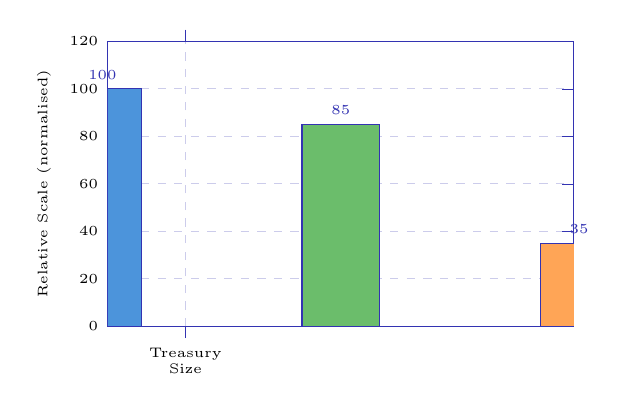
\begin{tikzpicture}
\begin{axis}[
  ybar,
  bar width=28pt,
  width=7.5cm,
  height=5.2cm,
  symbolic x coords={Treasury Size, DAO Count, Participation},
  xtick=data,
  xticklabels={Treasury\\Size, DAO\\Count, Governance\\Participation},
  xticklabel style={font=\tiny, text width=2.5cm, align=center},
  ymin=0, ymax=120,
  ytick={0,20,40,60,80,100,120},
  yticklabel style={font=\tiny},
  ylabel style={font=\tiny},
  ylabel={Relative Scale (normalised)},
  axis line style={draw=mlpurple},
  tick style={draw=mlpurple},
  nodes near coords,
  nodes near coords style={font=\tiny, color=mlpurple},
  point meta=y,
  enlarge x limits=0.25,
  grid=major,
  grid style={dashed, mllavender3},
]
\addplot[fill=mlblue!70,   draw=mlpurple] coordinates {(Treasury Size,   100)};
\addplot[fill=mlgreen!70,  draw=mlpurple] coordinates {(DAO Count,        85)};
\addplot[fill=mlorange!70, draw=mlpurple] coordinates {(Participation,    35)};
\end{axis}
\end{tikzpicture}
\end{column}
\begin{column}{0.36\textwidth}
\vspace{4mm}
\begin{block}{Key Metrics}
\begin{itemize}\setlength\itemsep{4pt}
  \item[\small$\checkmark$] \small \textbf{\$25B+} in DAO treasuries
  \item[\small$\checkmark$] \small \textbf{10,000+} DAOs created globally
  \item[\small$\checkmark$] \small \textbf{$<$10\%} average voter turnout
  \item[\small$\checkmark$] \small \textbf{50+} governance frameworks
\end{itemize}
\end{block}
\end{column}
\end{columns}
\bottomnote{DAOs control billions in assets yet face fundamental governance challenges: participation, accountability, and legal clarity.}
\end{frame}

% Frame 3: DAO Ecosystem at a Glance
\begin{frame}{DAO Ecosystem at a Glance}
\vspace{2mm}
\begin{center}
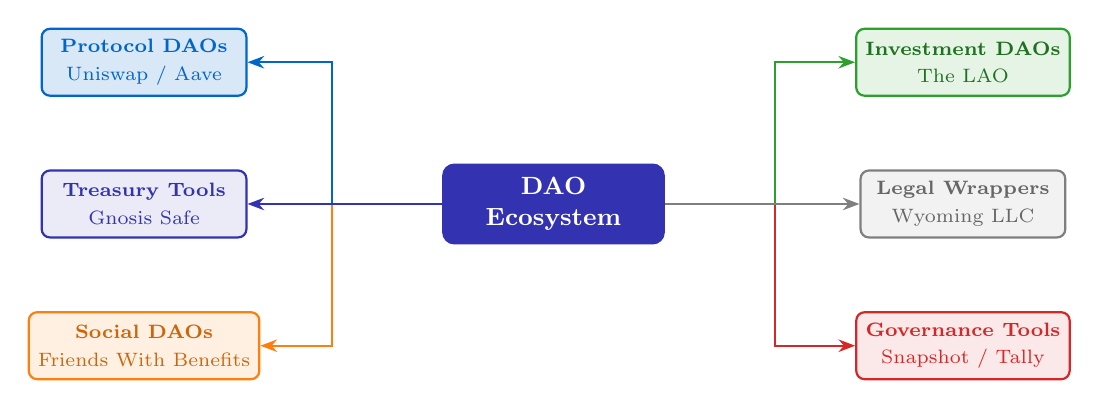
\begin{tikzpicture}[
  cbox/.style={rectangle, rounded corners=4pt, draw=mlpurple, thick,
               fill=mlpurple, minimum width=2.8cm, minimum height=1.0cm,
               font=\small\bfseries, align=center, text=white},
  sbox/.style={rectangle, rounded corners=3pt, thick,
               minimum width=2.6cm, minimum height=0.85cm,
               font=\scriptsize, align=center},
  arr/.style={-{Stealth[length=6pt]}, thick}
]
% Center node
\node[cbox] (center) at (0,0) {DAO\\Ecosystem};

% Spoke nodes
\node[sbox, draw=mlblue,   fill=mlblue!15,   text=mlblue]              (proto)  at (-5.2, 1.8)
  {\textbf{Protocol DAOs}\\[2pt]Uniswap / Aave};

\node[sbox, draw=mlgreen,  fill=mlgreen!12,  text=mlgreen!70!black]    (invest)  at ( 5.2, 1.8)
  {\textbf{Investment DAOs}\\[2pt]The LAO};

\node[sbox, draw=mlorange, fill=mlorange!12, text=mlorange!80!black]   (social) at (-5.2,-1.8)
  {\textbf{Social DAOs}\\[2pt]Friends With Benefits};

\node[sbox, draw=mlred,    fill=mlred!10,    text=mlred]               (gov)  at ( 5.2,-1.8)
  {\textbf{Governance Tools}\\[2pt]Snapshot / Tally};

\node[sbox, draw=mlpurple, fill=mlpurple!10, text=mlpurple]            (treas) at (-5.2, 0.0)
  {\textbf{Treasury Tools}\\[2pt]Gnosis Safe};

\node[sbox, draw=mlgray,   fill=mlgray!10,   text=mlgray!80!black]     (legal)  at ( 5.2, 0.0)
  {\textbf{Legal Wrappers}\\[2pt]Wyoming LLC};

% Arrows
\draw[arr, draw=mlblue]   (center.west) -- ++(-1.4,0) |- (proto.east);
\draw[arr, draw=mlgreen]  (center.east) -- ++(1.4,0)  |- (invest.west);
\draw[arr, draw=mlorange] (center.west) -- ++(-1.4,0) |- (social.east);
\draw[arr, draw=mlred]    (center.east) -- ++(1.4,0)  |- (gov.west);
\draw[arr, draw=mlpurple] (center.west) -- ++(-1.4,0) |- (treas.east);
\draw[arr, draw=mlgray]   (center.east) -- ++(1.4,0)  |- (legal.west);
\end{tikzpicture}
\end{center}
\bottomnote{The DAO ecosystem spans protocol governance, investment vehicles, social coordination, and supporting legal and tooling infrastructure.}
\end{frame}

% Frame 4: DAO Growth Trajectory
\begin{frame}{DAO Growth Trajectory}
\begin{columns}[T]
\begin{column}{0.62\textwidth}
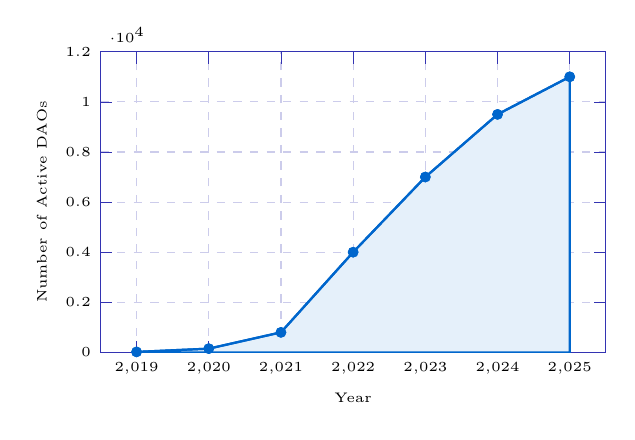
\begin{tikzpicture}
\begin{axis}[
  width=8.0cm,
  height=5.4cm,
  xmin=2018.5, xmax=2025.5,
  ymin=0, ymax=12000,
  xtick={2019,2020,2021,2022,2023,2024,2025},
  ytick={0,2000,4000,6000,8000,10000,12000},
  xticklabel style={font=\tiny},
  yticklabel style={font=\tiny},
  xlabel style={font=\tiny},
  ylabel style={font=\tiny},
  xlabel={Year},
  ylabel={Number of Active DAOs},
  axis line style={draw=mlpurple},
  tick style={draw=mlpurple},
  grid=major,
  grid style={dashed, mllavender3},
]
\addplot[color=mlblue, solid, thick, mark=*, mark size=1.5pt,
         fill=mlblue!10] coordinates {
  (2019,20)(2020,150)(2021,800)(2022,4000)(2023,7000)(2024,9500)(2025,11000)
} \closedcycle;
\addplot[color=mlblue, solid, thick, mark=*, mark size=1.5pt] coordinates {
  (2019,20)(2020,150)(2021,800)(2022,4000)(2023,7000)(2024,9500)(2025,11000)
};
\end{axis}
\end{tikzpicture}
\end{column}
\begin{column}{0.36\textwidth}
\vspace{4mm}
\begin{block}{Growth Drivers}
\begin{itemize}\setlength\itemsep{4pt}
  \item[\small$\checkmark$] \small \textbf{DeFi explosion} creating protocol governance needs
  \item[\small$\checkmark$] \small \textbf{Token governance} adoption at scale
  \item[\small$\checkmark$] \small \textbf{Legal recognition} in Wyoming and beyond
  \item[\small$\checkmark$] \small \textbf{Tooling maturity} lowering launch barriers
\end{itemize}
\end{block}
\end{column}
\end{columns}
\bottomnote{Active DAOs grew from under 50 in 2019 to over 10,000 by 2025, driven by DeFi adoption and maturing governance tooling.}
\end{frame}

% Frame 5: Course Coverage
\begin{frame}{Course Coverage}
\vspace{2mm}
\begin{center}
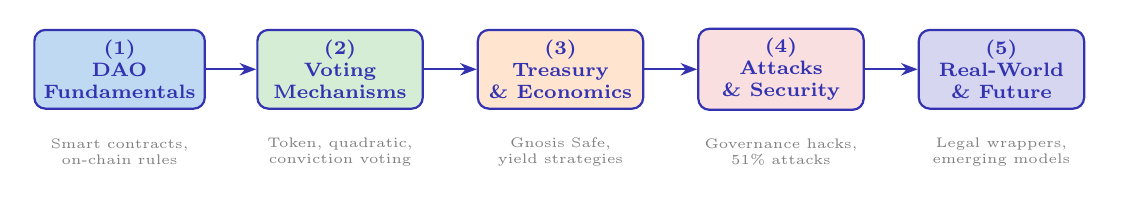
\begin{tikzpicture}[
  procstep/.style={
    rectangle, rounded corners=4pt,
    minimum width=2.1cm, minimum height=1.0cm,
    draw=mlpurple, thick,
    fill=mllavender3,
    font=\scriptsize\bfseries,
    align=center,
    text=mlpurple
  },
  conn/.style={-{Stealth[length=6pt]}, thick, draw=mlpurple}
]
\node[procstep, fill=mlblue!25]    (s1) at (0,0)    {(1)\\DAO\\Fundamentals};
\node[procstep, fill=mlgreen!20]   (s2) at (2.8,0)  {(2)\\Voting\\Mechanisms};
\node[procstep, fill=mlorange!20]  (s3) at (5.6,0)  {(3)\\Treasury\\\& Economics};
\node[procstep, fill=mlred!15]     (s4) at (8.4,0)  {(4)\\Attacks\\\& Security};
\node[procstep, fill=mlpurple!20]  (s5) at (11.2,0) {(5)\\Real-World\\\& Future};

\draw[conn] (s1) -- (s2);
\draw[conn] (s2) -- (s3);
\draw[conn] (s3) -- (s4);
\draw[conn] (s4) -- (s5);

\node[font=\tiny, text=mlgray, align=center, text width=2.1cm] at (0,-1.05)
  {Smart contracts,\\on-chain rules};
\node[font=\tiny, text=mlgray, align=center, text width=2.1cm] at (2.8,-1.05)
  {Token, quadratic,\\conviction voting};
\node[font=\tiny, text=mlgray, align=center, text width=2.1cm] at (5.6,-1.05)
  {Gnosis Safe,\\yield strategies};
\node[font=\tiny, text=mlgray, align=center, text width=2.1cm] at (8.4,-1.05)
  {Governance hacks,\\51\% attacks};
\node[font=\tiny, text=mlgray, align=center, text width=2.1cm] at (11.2,-1.05)
  {Legal wrappers,\\emerging models};
\end{tikzpicture}
\end{center}
\vspace{4mm}
\begin{columns}[T]
\begin{column}{0.48\textwidth}
\begin{block}{Prerequisites}
\begin{itemize}\setlength\itemsep{2pt}
  \item[\small$\checkmark$] \small Basic blockchain and smart contract knowledge
  \item[\small$\checkmark$] \small Introductory DeFi and token concepts
\end{itemize}
\end{block}
\end{column}
\begin{column}{0.48\textwidth}
\begin{block}{Outcomes}
\begin{itemize}\setlength\itemsep{2pt}
  \item[\small$\checkmark$] \small Design and evaluate DAO governance structures
  \item[\small$\checkmark$] \small Identify attack vectors and security trade-offs
\end{itemize}
\end{block}
\end{column}
\end{columns}
\bottomnote{From on-chain fundamentals to real-world deployment in five interconnected modules covering design, security, and law.}
\end{frame}

% Frame 6: What You Will Learn
\begin{frame}{What You Will Learn}
\begin{columns}[T]
\begin{column}{0.44\textwidth}
\vspace{2mm}
\begin{block}{Learning Outcomes}
\begin{itemize}\setlength\itemsep{5pt}
  \item[\small$\checkmark$] \small \textbf{DAO architecture} --- smart contract structure, proposal and execution lifecycle
  \item[\small$\checkmark$] \small \textbf{Voting mechanisms} --- token voting, quadratic voting, conviction voting trade-offs
  \item[\small$\checkmark$] \small \textbf{Treasury management} --- multisig custody, yield strategies, budget governance
  \item[\small$\checkmark$] \small \textbf{Attack vectors} --- governance exploits, flash-loan attacks, Sybil resistance
  \item[\small$\checkmark$] \small \textbf{Best practices} --- participation incentives, legal wrappers, tooling selection
\end{itemize}
\end{block}
\end{column}
\begin{column}{0.54\textwidth}
\vspace{2mm}
\begin{center}
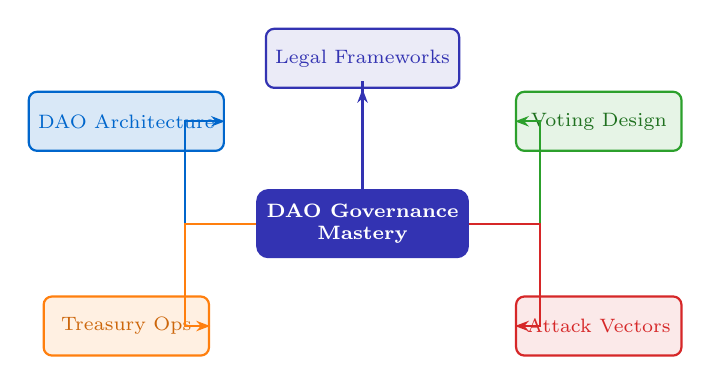
\begin{tikzpicture}[
  cbox/.style={rectangle, rounded corners=4pt, draw=mlpurple, thick,
               fill=mlpurple, minimum width=2.6cm, minimum height=0.85cm,
               font=\scriptsize\bfseries, align=center, text=white},
  fbox/.style={rectangle, rounded corners=3pt, thick,
               minimum width=2.1cm, minimum height=0.75cm,
               font=\scriptsize, align=center},
  farr/.style={-{Stealth[length=5pt]}, thick}
]
% Central node
\node[cbox] (nm) at (0,0) {DAO Governance\\Mastery};

% Skill nodes
\node[fbox, draw=mlblue,   fill=mlblue!15,   text=mlblue]              (arch) at (-3.0, 1.3) {DAO Architecture};
\node[fbox, draw=mlgreen,  fill=mlgreen!12,  text=mlgreen!70!black]    (vote) at ( 3.0, 1.3) {Voting Design};
\node[fbox, draw=mlorange, fill=mlorange!12, text=mlorange!80!black]   (tres) at (-3.0,-1.3) {Treasury Ops};
\node[fbox, draw=mlred,    fill=mlred!10,    text=mlred]               (atk)  at ( 3.0,-1.3) {Attack Vectors};
\node[fbox, draw=mlpurple, fill=mlpurple!10, text=mlpurple]            (leg)  at ( 0.0, 2.1) {Legal Frameworks};

% Arrows
\draw[farr, draw=mlblue]   (nm.west)  -- ++(-0.9,0) |- (arch.east);
\draw[farr, draw=mlgreen]  (nm.east)  -- ++(0.9,0)  |- (vote.west);
\draw[farr, draw=mlorange] (nm.west)  -- ++(-0.9,0) |- (tres.east);
\draw[farr, draw=mlred]    (nm.east)  -- ++(0.9,0)  |- (atk.west);
\draw[farr, draw=mlpurple] (nm.north) -- ++(0,0.6)  |- (leg.south);
\end{tikzpicture}
\end{center}
\end{column}
\end{columns}
\vspace{1mm}
\bottomnote{By the end you will be able to design, evaluate, and secure DAO governance systems with rigorous on-chain and off-chain knowledge.}
\end{frame}

\end{document}
